% USE XeLaTeX

\documentclass{beamer}
%% Possible paper sizes: a0, a0b, a1, a2, a3, a4.
%% Possible orientations: portrait, landscape
%% Font sizes can be changed using the scale option.
\usepackage[size=a1,orientation=portrait,scale=1.1]{beamerposter}


\usepackage[utf8]{inputenc}
\usepackage[T1]{fontenc}
\usepackage{libertine}
\usepackage[scaled=0.92]{inconsolata}
\usepackage[libertine]{newtxmath}


%% packages added by GG
\setbeamertemplate{caption}[numbered]  % enable numbering of figures in beamer-poster

\usepackage{lipsum,lineno}

\usepackage{multicol}
\usepackage{amsmath, amsthm, amsfonts}
\usepackage{amsfonts}
\usepackage{xcolor}
\usepackage{mathbbol}
\usepackage{amssymb}             % AMS Math
\DeclareSymbolFontAlphabet{\amsmathbb}{AMSb}%
\usepackage{bbm}


\usepackage{caption}
\usepackage{graphicx,subfigure}
\usepackage{floatrow}
\usepackage{booktabs} % more pro tables
\usepackage{tabularx} % tables for boundary conditions
\usepackage{multirow} % enchanted tables 
\usepackage[shortlabels]{enumitem} % support letters for enumeration

%% GG styles

\newenvironment<>{redblock}[1]{
  \setbeamercolor{block title}{fg=white,bg=red!75!black}
  \setbeamercolor{block body}{fg=black,bg=white!25!red}
  \begin{block}#2{#1}}{\end{block}}
  
\newenvironment<>{blueblock}[1]{%
  \setbeamercolor{block title}{fg=white,bg=blue!75!black}%
  \begin{block}#2{#1}}{\end{block}}
  
\newenvironment<>{greenblock}[1]{%
  \setbeamercolor{block title}{fg=white,bg=green!50!black}%
  \begin{block}#2{#1}}{\end{block}}
  
%% end of GG stuff

\definecolor{VioletRed}{RGB}
%{127,127,127}% ccfd-grey
{0,26,102} % pw-blue
%{215, 0, 0} % red
\setbeamercolor{block title}{fg=VioletRed,bg=white}
\setbeamercolor{block body}{fg=black,bg=white}
\setbeamercolor{local structure}{fg=VioletRed}
\setbeamercolor{bibliography structure}{fg=VioletRed}
\setbeamercolor{bibliography item}{fg=black,bg=white}
\setbeamercolor{bibliography entry author}{fg=black,bg=white}
\setbeamercolor{bibliography item}{fg=black,bg=white}
\setbeamercolor{bibliography entry location}{fg=black} 
\setbeamercolor{bibliography entry note}{fg=black} 

\newenvironment<>{varblock}[2][\textwidth]{%
   \setlength{\textwidth}{#1}
   \begin{actionenv}#3%
     \def\insertblocktitle{#2}%
     \par%
     \usebeamertemplate{block begin}}
   {\par%
     \usebeamertemplate{block end}%
   \end{actionenv}}
   

\author[ggruszczynski@meil.pw.edu.pl]{G. Gruszczyński, Ł. Łaniewski-Wołłk%, J. Szumbarski 
%\\ \texttt{sam@somewhere.edu}
}
%\author[sam \& joey]
%       {\parbox[t]{1.5in}{sam \\ \texttt{sam@somewhere.edu}} \and 
%        \parbox[t]{1.5in}{joey}
%       }
%ggruszczynski@meil.pw.edu.pl

\institute{Institute of Aeronautics and Applied Mechanics \\
Warsaw University of Technology, Warszawa, Poland}

\subtitle{Numerical modelling \\ of Super Hydrophobic Surfaces \\
Using Lattice Boltzmann method}

\addtobeamertemplate{headline}{} {
 \leavevmode
  \begin{columns}[T]
    \begin{column}{.15\linewidth}
        \vskip2cm
        \hskip1cm
        \hspace*{4.0em}
        
\includegraphics[width=1.2\linewidth]{Images/LOGO/ccfd3.png}
    \end{column}
    \begin{column}{.7\linewidth}
         \vskip2cm
         \centering
         \usebeamercolor{title in headline}{\color{black}\Huge{\textbf{\inserttitle}}\\[0.5ex]}
         \vskip.5cm
         \usebeamercolor{subtitle in headline}{\color{black}\huge{\insertsubtitle}\\[0.5ex]}
         \vskip.5cm
         \usebeamercolor{author in headline}{\color{fg}\Large{\textbf{\insertauthor}}\\[1ex]}
         \usebeamercolor{institute in headline}{\color{fg}\large{\insertinstitute}\\[1ex]}
         \vskip1cm
    \end{column}
    \begin{column}{.15\linewidth}
        \vskip 2.1cm
        \begin{flushleft}
        \hspace*{6.5em}
        
\includegraphics[width=0.6\linewidth]{Images/LOGO/symbol-PW.pdf}
        \end{flushleft}
        \hskip1cm
    \end{column}        
   \vspace{1cm}
  \end{columns}
 \vspace{0.5in}
 \hspace{0.5in}\begin{beamercolorbox}[wd=47in,colsep=0.15cm]{black}\end{beamercolorbox}
 \vspace{0.1in}
}
\usepackage{hyperref}
\usepackage{cleveref}
\begin{document}
\begin{frame}[fragile]\centering

%%%%%%%%%%%%%%%%%%%%%%%% No Columns - Intro %%%%%%%%%%%%%%%%%%%%%%%%
\begin{columns}[T]
\begin{column}{.96\textwidth}
\begin{block}{Introduction}
Super Hydrophobic Surfaces (SHS) have been of interest to researchers for many years, because of their ability to reduce drag and maintain the surface to be dry and clean, and a large variety of methods have been applied to study their phenomena. 
The lattice Boltzmann method, thanks to its mesoscopic nature is a suitable candidate to simulate the intermolecular interactions responsible for the interfacial flows in a microscale. 
In this contribution, we present a conservative, phase-field model for simulation of immiscible multiphase flows using an incompressible, velocity based Cascaded Lattice Boltzmann Method. 
As a study case, we present a simulation of an SHS.
%Generally, the super hydrophobic effect comes from both chemical interaction and surface shape in a microscale.
%The principle of work is based on the fact, that the tiny air-bubbles are entrapped into the microstructure of the surface being in the contact with fluids which is sliding on them. 
%Unfortunately, usage of SHS depends on the flow condition. 
%It may happen, that too fast flow or improper shape of the surface would cause the air-bubbles to wash out and to loose the desired properties. \\

%Multiphase flows are challenging due to complex dynamics involved in phase change or segregation and in the tracking of the interface between different fluids. 
%The lattice Boltzmann method, thanks to its mesoscopic nature is a suitable candidate to simulate the intermolecular interactions responsible for the interfacial flows in a microscale. 
%Additionally, the LBM is easy in implementation and inability of handling complex geometries such as porous media or surface roughness. 
%Computations are performed locally, thus the algorithm can be parallelized in a straightforward manner. 
%These features resulted in rising popularity and commercial success of the method. 
%Application of the LB method to the simulation of SHS is a recent research field. 
\end{block}

\end{column}
\end{columns}

\begin{columns}[T]
%\begin{column}{.2975\textwidth}
\begin{column}{.32\textwidth}

\begin{block}{How SHS works?}
\begin{multicols}{2}
\begin{figure}[H]
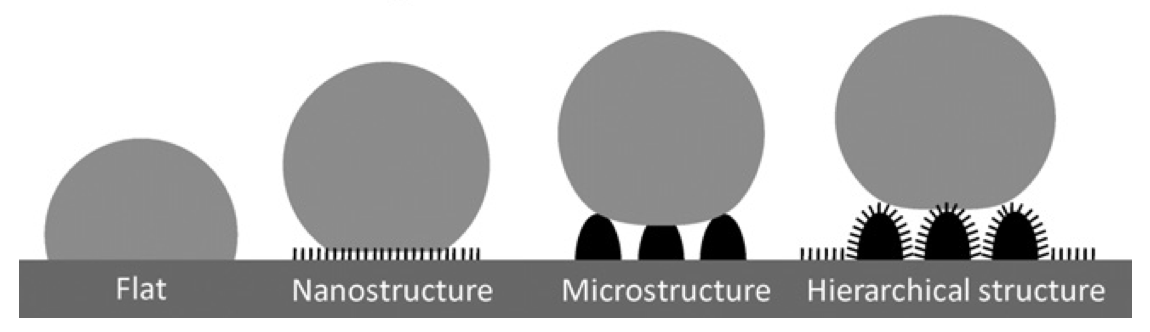
\includegraphics[width = 1 \textwidth]{Images/shs_structure.png} 
\caption{Surface structure}
\end{figure}
\columnbreak 
\begin{figure}[H]
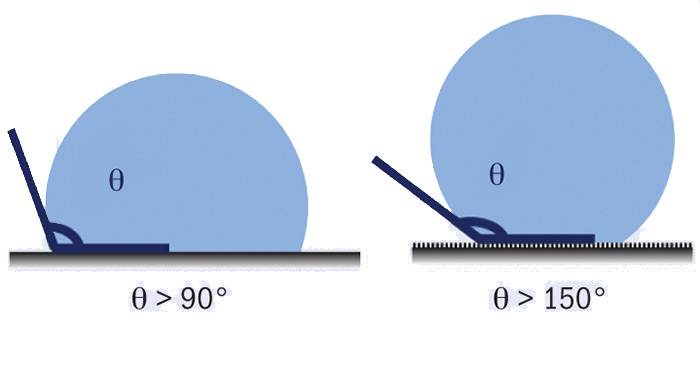
\includegraphics[width = 1 \textwidth]{Images/chemical_n_shape.jpg} 
\caption{Coating vs structure}
\end{figure}
\end{multicols}
Generally, the super hydrophobic effect comes from both chemical interaction and surface shape in a microscale.
The principle of work is based on the fact, that the tiny air-bubbles are entrapped into the microstructure of the surface being in the contact with fluids which is sliding on them. 
Unfortunately, usage of SHS depends on the flow condition. 
It may happen, that too fast flow or improper shape of the surface would cause the air-bubbles to wash out and to loose the desired properties.\\
Chemical surface treatment can results in contact angles up to 120$^\circ$. \,% \cite{Blossey2003}. 
Higher values observed in a macro scale can be achieved only by additional micro roughing of the surface.
%The super hydrophobic effect origins from both surface shape and coating (chemical composition).
%Generally, the super hydrophobic effect comes from both chemical interaction and surface shape in a microscale. 
%The principle of work is based on the fact, that the tiny air-bubbles are entrapped into the microstructure of the surface being in the contact with fluids which is sliding on them. Unfortunately, usage of SHS depends on the flow condition. 
%It may happen, that too fast flow or improper shape of the surface would cause the air-bubbles to wash out and to loose the desired properties. \\
\end{block}

\begin{block}{How SHS looks like?}
\begin{multicols}{2}
\begin{figure}[H]
   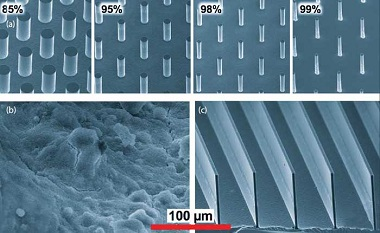
\includegraphics[width= 1 \textwidth]{Images/human_SHS.jpg} 
   \caption{Manufactured}
\end{figure}
\columnbreak 
\begin{figure}[H]
   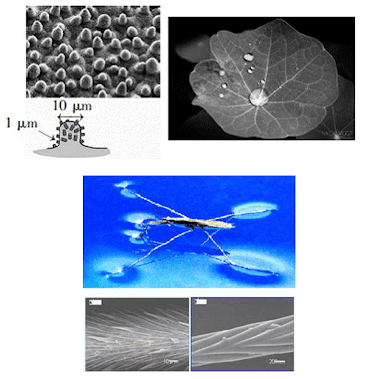
\includegraphics[width= 1 \textwidth]{Images/natural_SHS.png} 
   \caption{Natural}
\end{figure}
\end{multicols}
To support a thin layer of air, an array of posts or ridges is usually applied.
Such symmetric structures are expensive to manufacture, fragile and not common in nature. 
However, experiments have shown that an unstructured, rough surface can work as well as regularly spaced arrays of ridges or posts.
%Gogte et al. \cite{Gogte2005} showed that an unstructured rough surface can work as well as regularly spaced arrays of ridges or posts. Later, an analytical model was developed by  Nosonovsky and Bhushan \cite{Nosonovsky2007a}. 
%Due to its mesoscale nature, LBM can easily capture the effect of random roughness.
%It has been successfully applied by Kuner and Harting \cite{Kunert2008} to study effective wall position. More recently, Yuan and Zhang \cite{Yuan2017} investigated droplets impacting a randomly distributed rough surface.
\end{block}


\end{column}

%\begin{column}{.2975\textwidth}
\begin{column}{.605 \textwidth}
\begin{block}{Governing Equations}
We simulate an incompressible, non-miscible, multiphase flow.
\begin{multicols}{2}
\textbf{Hydrodynamics}\\
The continuity and momentum equations are,
\begin{eqnarray}  
\left\{
    \begin{array}{ll}
\frac{\partial \rho}{\partial t} + \nabla \cdot \rho \textbf{u} = 0 \\
\rho\left( \frac{\partial \textbf{u} }{\partial t} + \textbf{u} \cdot \nabla \textbf{u}\right) = -\nabla p + \nabla \cdot (\mu[ \nabla \textbf{u} + (\nabla \textbf{u})^\top]) + \textbf{F}_s + \textbf{F}_b .
    \end{array}\nonumber 
\right.
\end{eqnarray}
Forcing terms are given as,
\begin{eqnarray}  
     \boldsymbol{F}_s = \mu_{\phi}\nabla \phi                 \hspace{1.5em};\hspace{1.5em} 
     \boldsymbol{F}_b = [G_X, G_Y]^\top . \nonumber
\end{eqnarray} 

\columnbreak 

\textbf{Phase-field}\\
Interface tracking is realized using the phase-field approach,
\begin{eqnarray}
\frac{\partial \phi}{\partial t} + \nabla \cdot \phi \textbf{u}
=
\nabla \cdot M
\left( 
\nabla \phi - 
  %\underbrace{
  \frac{\nabla \phi}{|\nabla \phi|} \frac{[1-4(\phi - \phi_0)^2]}{\gamma} 
  %}_{Force \, term} 
\right). \nonumber
\end{eqnarray}
The interface is located in $ \phi_0 =(\phi_H + \phi_L)/2  $. \\
Density is a linear interpolation between $\rho_H$ and $\rho_L$,
\begin{eqnarray}
\rho = \rho_L +  \frac{\phi - \phi_L}{\phi_H - \phi_L}(\rho_H -\rho_L).  \nonumber
\end{eqnarray}
`Advection - Diffusion` of  $\phi$ is solved on a separate D2Q9 lattice.% \\ \vspace{1.5em}
\end{multicols}
\end{block}

\begin{block}{Lattice Boltzmann Method - Algorithm}
\begin{multicols}{2}
The raw moments and central moments are defined as,
\begin{eqnarray}
\Upsilon_{mn} &=& \sum_{\alpha}(e_{\alpha x})^m ( e_{\alpha y})^n f_{\alpha} \nonumber \label{eq:raw_mom_def} \\
\tilde{\Upsilon}_{mn} &=& \sum_{\alpha} ( e_{\alpha x} - u_x)^m ( e_{\alpha y} - u_y)^n f_{\alpha} \nonumber \label{eq:cm_mom_def}
\end{eqnarray}
Pressure and velocity are interpreted as zeroth and first moment respectively,
\begin{eqnarray} 
p^{*} &=& \Upsilon_{00} = \sum_\alpha f_\alpha,  \nonumber % \hspace{2em} \text{- normalized pressure} 
 \\
\textbf{u} &=& [u_x, u_y]^\top = [ \Upsilon_{10}, \Upsilon_{01}]^\top 
= \sum_\alpha f_\alpha \textbf{e}_\alpha + \frac{\textbf{F}}{2 \rho} \delta t. \nonumber 
% \hspace{2em} \text{- macroscopic velocity} 
\end{eqnarray}
\columnbreak
\begin{figure}[H]
   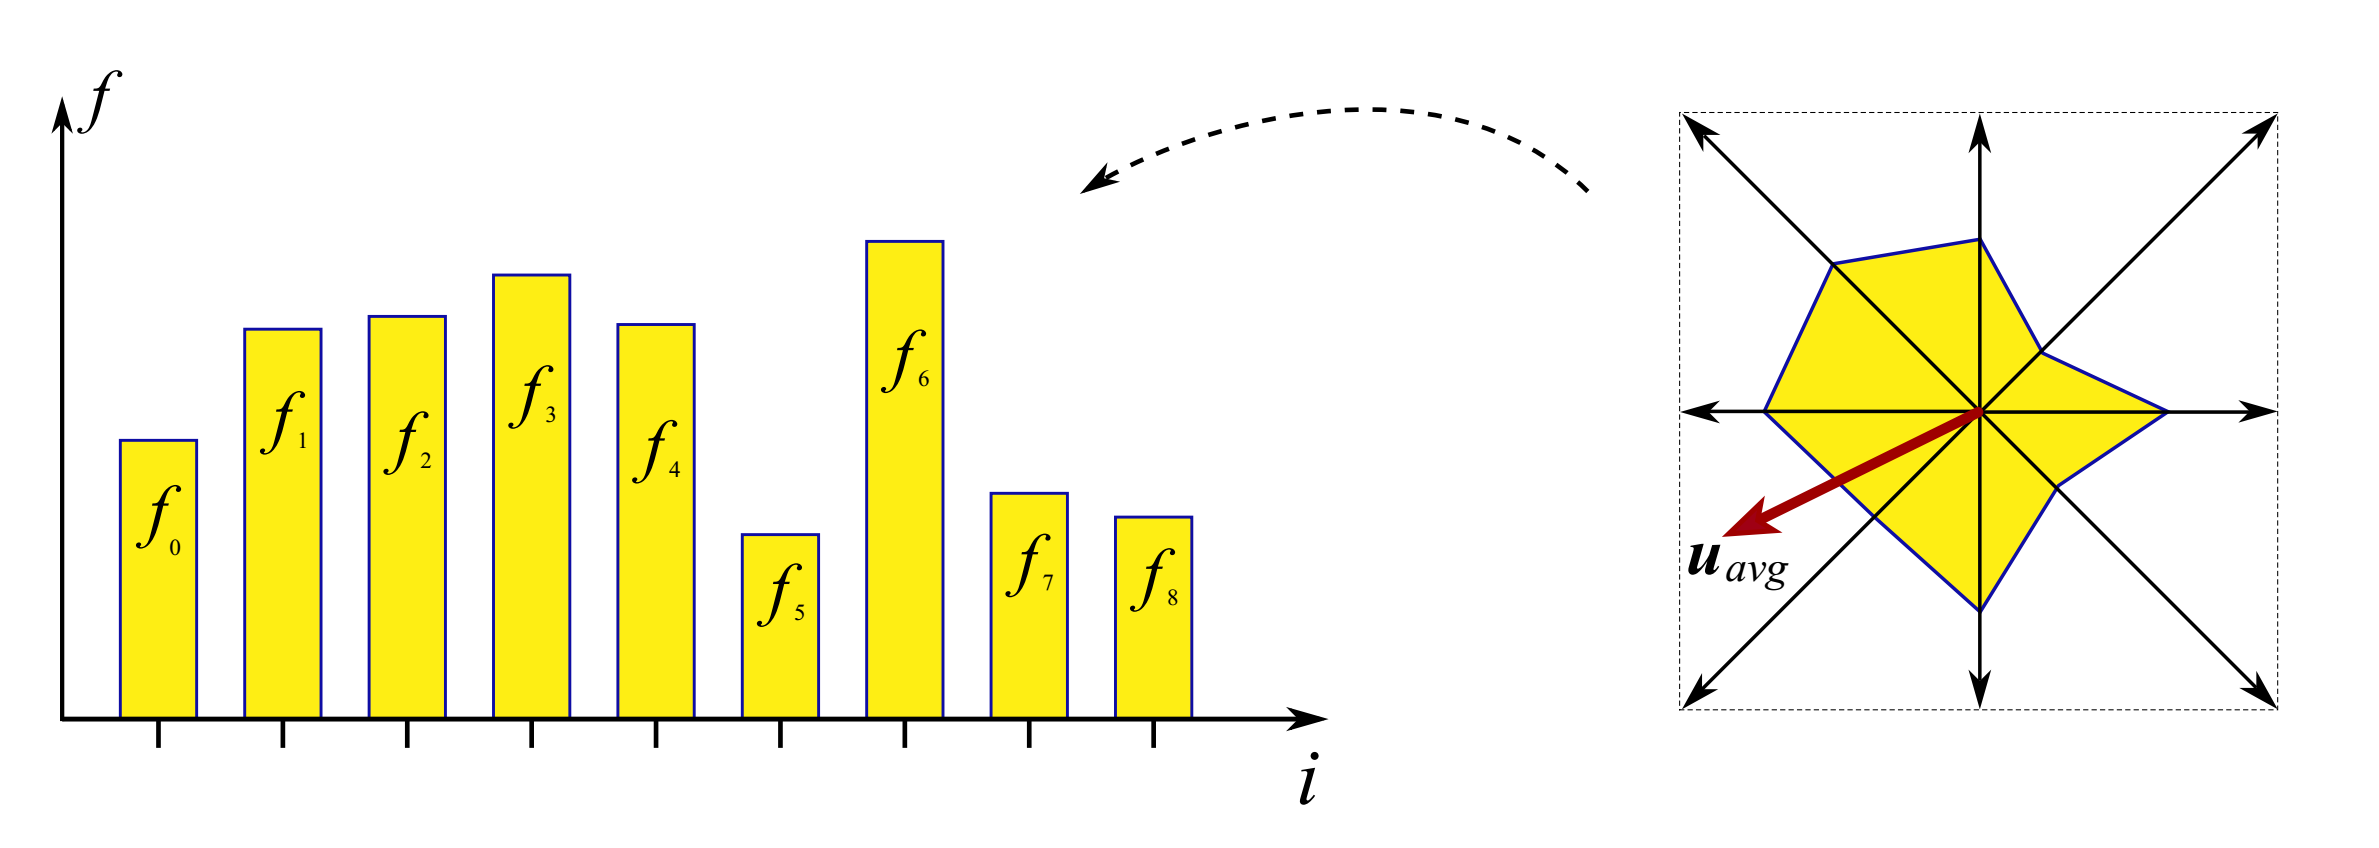
\includegraphics[width= 1 \textwidth]{Images/latticeVelocities_concept.png} 
   \caption{Concept of lattice velocities}
   \label{fig:latticeVelocities_concept}
\end{figure}
\end{multicols}

%The simplest, single relaxation scheme reads:
%
%\begin{multicols}{2}
%\begin{eqnarray} 
%  \underbrace{ f_i(\boldsymbol{x}+ \boldsymbol{e_i} \Delta {\boldsymbol{x}}, t +  \Delta {t} ) }_{Streaming} =
%  \underbrace{ f_i(\boldsymbol{x}, t ) - \frac{1}{\tau } ( f_i - f_i^{eq}) + F_i(\boldsymbol{x}, t ) }_{Collision} \nonumber
%\end{eqnarray}
%\begin{itemize}
%\item  $\tau = \tau(\nu)$ relaxation parameter, $\nu$ is the kinematic viscosity 
%\item $f_i$ - discrete probability distribution function
%\item $F_i$ - source term (ex. gravity force)
%\end{itemize}
%\columnbreak
%\begin{figure}[H]
%   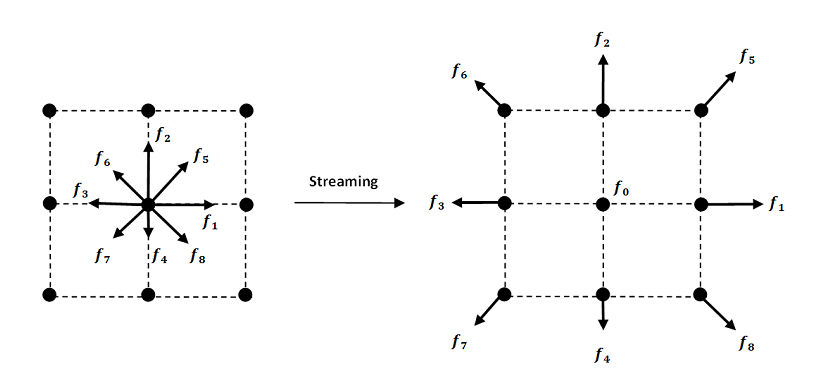
\includegraphics[width= 1 \textwidth]{Images/streaming.png} 
%   \caption{D2Q9: Streaming}
%   \label{fig:Streaming}
%\end{figure}
%\begin{figure}[H]
%   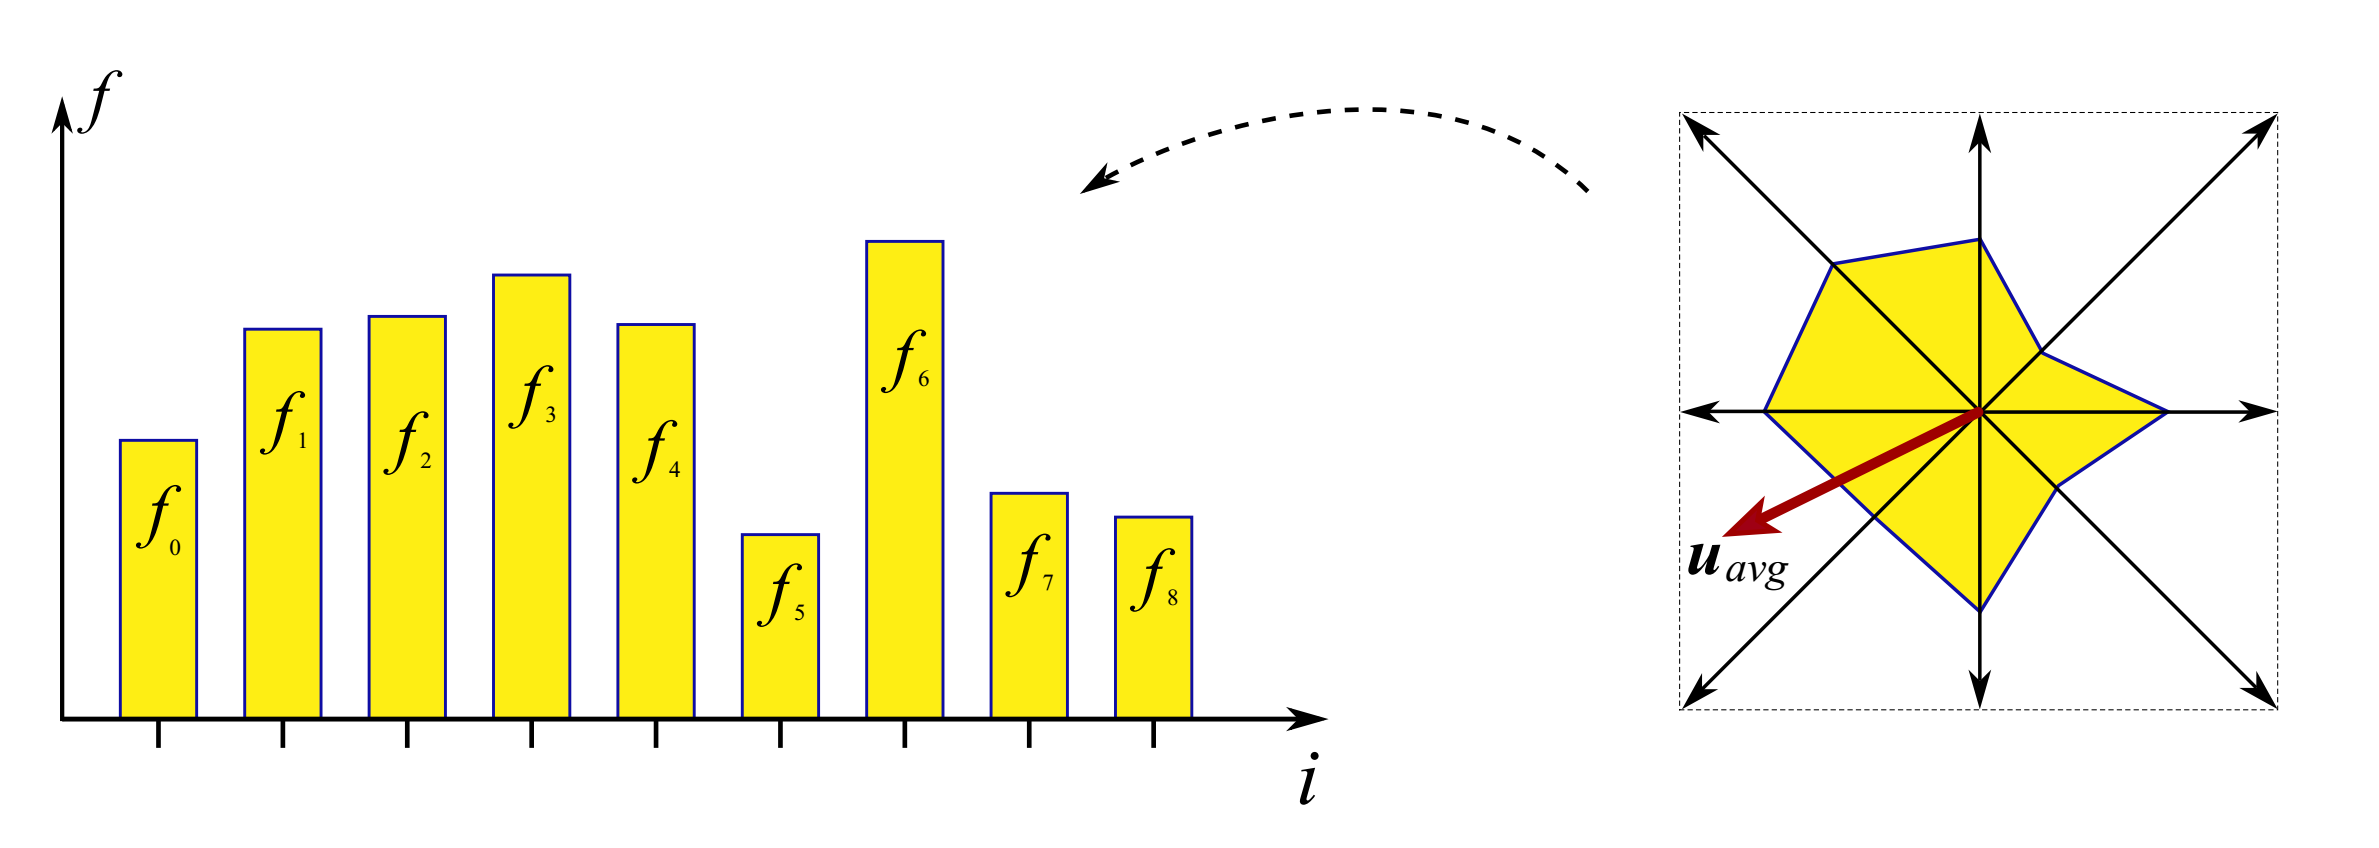
\includegraphics[width= 1 \textwidth]{Images/latticeVelocities_concept.png} 
%   \caption{Concept of lattice velocities}
%   \label{fig:latticeVelocities_concept}
%\end{figure}
%\end{multicols}

We introduce improvements to the LB equations for interface tracking and incompressible hydrodynamics, by transforming the operations into the central moment space. 
The relaxation of central moments is defined in a reference frame moving with the fluid. %, while the commonly used multiple-relaxation time scheme performs collision in a fixed reference frame. 
As a consequence, Galilean invariance and stability of the method is improved.
\begin{multicols}{2}
\textbf{Hydrodynamics}\\
\textit{1} Initialize $ \boldsymbol{f}(\textbf{x}, t)  $, \\ \vspace{1.em}

\textit{2} Compute 
$\textbf{u} = [u_x, u_y]^\top = [ k_{10}, k_{01}]^\top 
= \sum_\alpha f_\alpha \textbf{e}_\alpha + \frac{\textbf{F}}{2 \rho} \delta t \nonumber  $, \\ \vspace{1.em}

\textit{3} Compute \linebreak
$\boldsymbol{\tilde{\Upsilon}}(\boldsymbol{x},t)
=\mathbb{N}\mathbb{M}\textbf{f}(\boldsymbol{x},t)$, 
\hspace{1em}
$\boldsymbol{\tilde{\Upsilon}}^{eq}(\boldsymbol{x},t)=$..., \hspace{1em} 
$\tilde{\textbf{F}}(\boldsymbol{x},t)=$...,
\\ \vspace{1.em}
 
\textit{4} Collision  \linebreak
$\boldsymbol{\tilde{\Upsilon}}^{*}(\textbf{x}, t) =  
(\mathbbm{1} - \mathbb{S})\boldsymbol{\tilde{\Upsilon}} + \mathbb{S} \boldsymbol{\tilde{\Upsilon}}^{eq}  + (\mathbbm{1} - \mathbb{S}/2)\tilde{\textbf{F}}, 
$
\\ \vspace{1.em}

\textit{5} Streaming  \linebreak
$
\boldsymbol{f}(\textbf{x} + \textbf{e}\delta t, t + \delta t ) 
= \mathbb{M}^{-1} \mathbb{N}^{-1} \boldsymbol{\tilde{\Upsilon}}^{*}(\textbf{x}, t).
$ 

%\end{block}
%\end{column}
%
%\begin{column}{.2975\textwidth}

%\begin{block}{Advection-diffusion equation revisited}
%The separation flux, $\textbf{j}_S$, is supposed to counteract the diffusion and reach a predefined interface profile in the equilibrium state:
%\begin{eqnarray}
%\frac{\partial \phi}{\partial t} + \nabla \cdot \phi \textbf{u}
%=
%\nabla \cdot (  
%  \underbrace{ M \nabla \phi }_{\textbf{j}_D}
% - \textbf{j}_S
%) \nonumber
%\end{eqnarray}
%Let us use a $tanh$ to smooth the step interface:
%\begin{eqnarray}
%\phi^{eq} = \frac{1}{2} tanh
%\left(
%\frac{2(\textbf{x} - \textbf{x}_0) }{\gamma}
%\right) \nonumber
%\end{eqnarray}
%Evaluate diffusive flux in the equilibrium:
%\begin{align*}
%\textbf{j}_D^{eq} &= M \nabla 
%\overbrace{
%\left[ \frac{1}{2} tanh \left(
%\frac{2(\textbf{x} - \textbf{x}_0) }{\gamma}
%\right) \right] }^{\phi^{eq}} 
%=  \frac{M}{2} \textbf{n} \frac{ \partial }{ \partial \textbf{x}_n}
%tanh \left[ \left(
%\frac{2(\textbf{x} - \textbf{x}_0) }{\gamma}
%\right) \right]  \\[1 em]
%&= \frac{M}{\gamma}  \textbf{n} 
%\underbrace{
%\left[  1 - 
%tanh^2  \left( \frac{2(\textbf{x} - \textbf{x}_0) }{\gamma}
%\right) \right] 
%}_{1 - 4 (\phi^{eq})^2 }
%\end{align*}
%Therefore:
%\begin{align*}
%\textbf{j}_S = M \textbf{n}
%%\underbrace{ \frac{\nabla \phi}{|\nabla \phi|}}_{\textbf{n}} 
%\frac{1 - 4 \phi^2}{\gamma}  \hspace{2 em}  where  \hspace{1 em} \textbf{n} = \frac{\nabla \phi}{|\nabla \phi|}
%\end{align*}
%\end{block}

%\begin{block}{Phase field}%

%\end{block}

%\begin{block}{Algorithm: phase-field}
\columnbreak 
\textbf{Phase-field}\\
\textit{1} Initialize 
$ \boldsymbol{h}(\textbf{x}, t) $, \\ \vspace{1.em}
%\pause

\textit{2} % Use $ \boldsymbol{u}$ from hydrodynamics,  \\ \vspace{1.em}
Compute $ \phi = \sum_{\alpha} h_{\alpha}(\boldsymbol{x},t) $ \\ \vspace{1.em}%


\textit{3} Compute \linebreak
$\boldsymbol{\tilde{\Upsilon}}^{\phi}(\boldsymbol{x},t)
=\mathbb{N}\mathbb{M}\textbf{h}(\boldsymbol{x},t)$,
\hspace{1em}
$\boldsymbol{\tilde{\Upsilon}}^{\phi,eq}(\boldsymbol{x},t)=$..., \hspace{1em}
$\tilde{\textbf{F}}^{\phi}(\boldsymbol{x},t)=$...,
\\ \vspace{1.em}
 
%%\pause
\textit{4} Collision \linebreak
%$ h_i ^{out}(\boldsymbol{x},t) = h_i^{in}(\boldsymbol{x},t) - \frac{1}{\tau_T} \bigg[ h_i^{in}(\boldsymbol{x},t) - h_i^{eq}(\boldsymbol{x},t) \bigg] + F_i^{\phi}(\boldsymbol{x}, t ) $
$ \boldsymbol{\tilde{\Upsilon}}^{\phi,*}(\textbf{x}, t) = 
(\mathbbm{1} - \mathbb{S}^{\phi}) \boldsymbol{\tilde{\Upsilon}}^\phi + \mathbb{S}^{\phi} \boldsymbol{\tilde{\Upsilon}}^{\phi, eq}  + 
(\mathbbm{1} - \mathbb{S}^{\phi}/2)
\tilde{\textbf{F}}^\phi,
$ 
\\ \vspace{1.em}
%
\textit{5} Streaming  \\
$
\boldsymbol{h}(\textbf{x} + \textbf{e}\delta t, t + \delta t ) 
= \mathbb{M}^{-1} \mathbb{N}^{-1} \boldsymbol{\tilde{\Upsilon}}^{\phi,*}(\textbf{x}, t).
$
%\end{block}
\end{multicols}
\end{block}
\end{column}
\end{columns}

\begin{columns}[T]
\begin{column}{.465\textwidth}

\begin{block}{Benchmarks}
%How SHS works $ \backsim $ two phase Coutte flow
%Match dynamic viscosity ratio to achieve the same effect as in the case of air-water interface:
%\begin{eqnarray}
%\mu^*=\frac{\nu_H \rho_H}{\nu_L \rho_L} = \frac{10^{-6} \cdot 1000}{1.5 \cdot 10^{-5} \cdot 1.22}= 54.6 \nonumber
%\end{eqnarray}
\begin{multicols}{2}
\begin{figure}[H]
   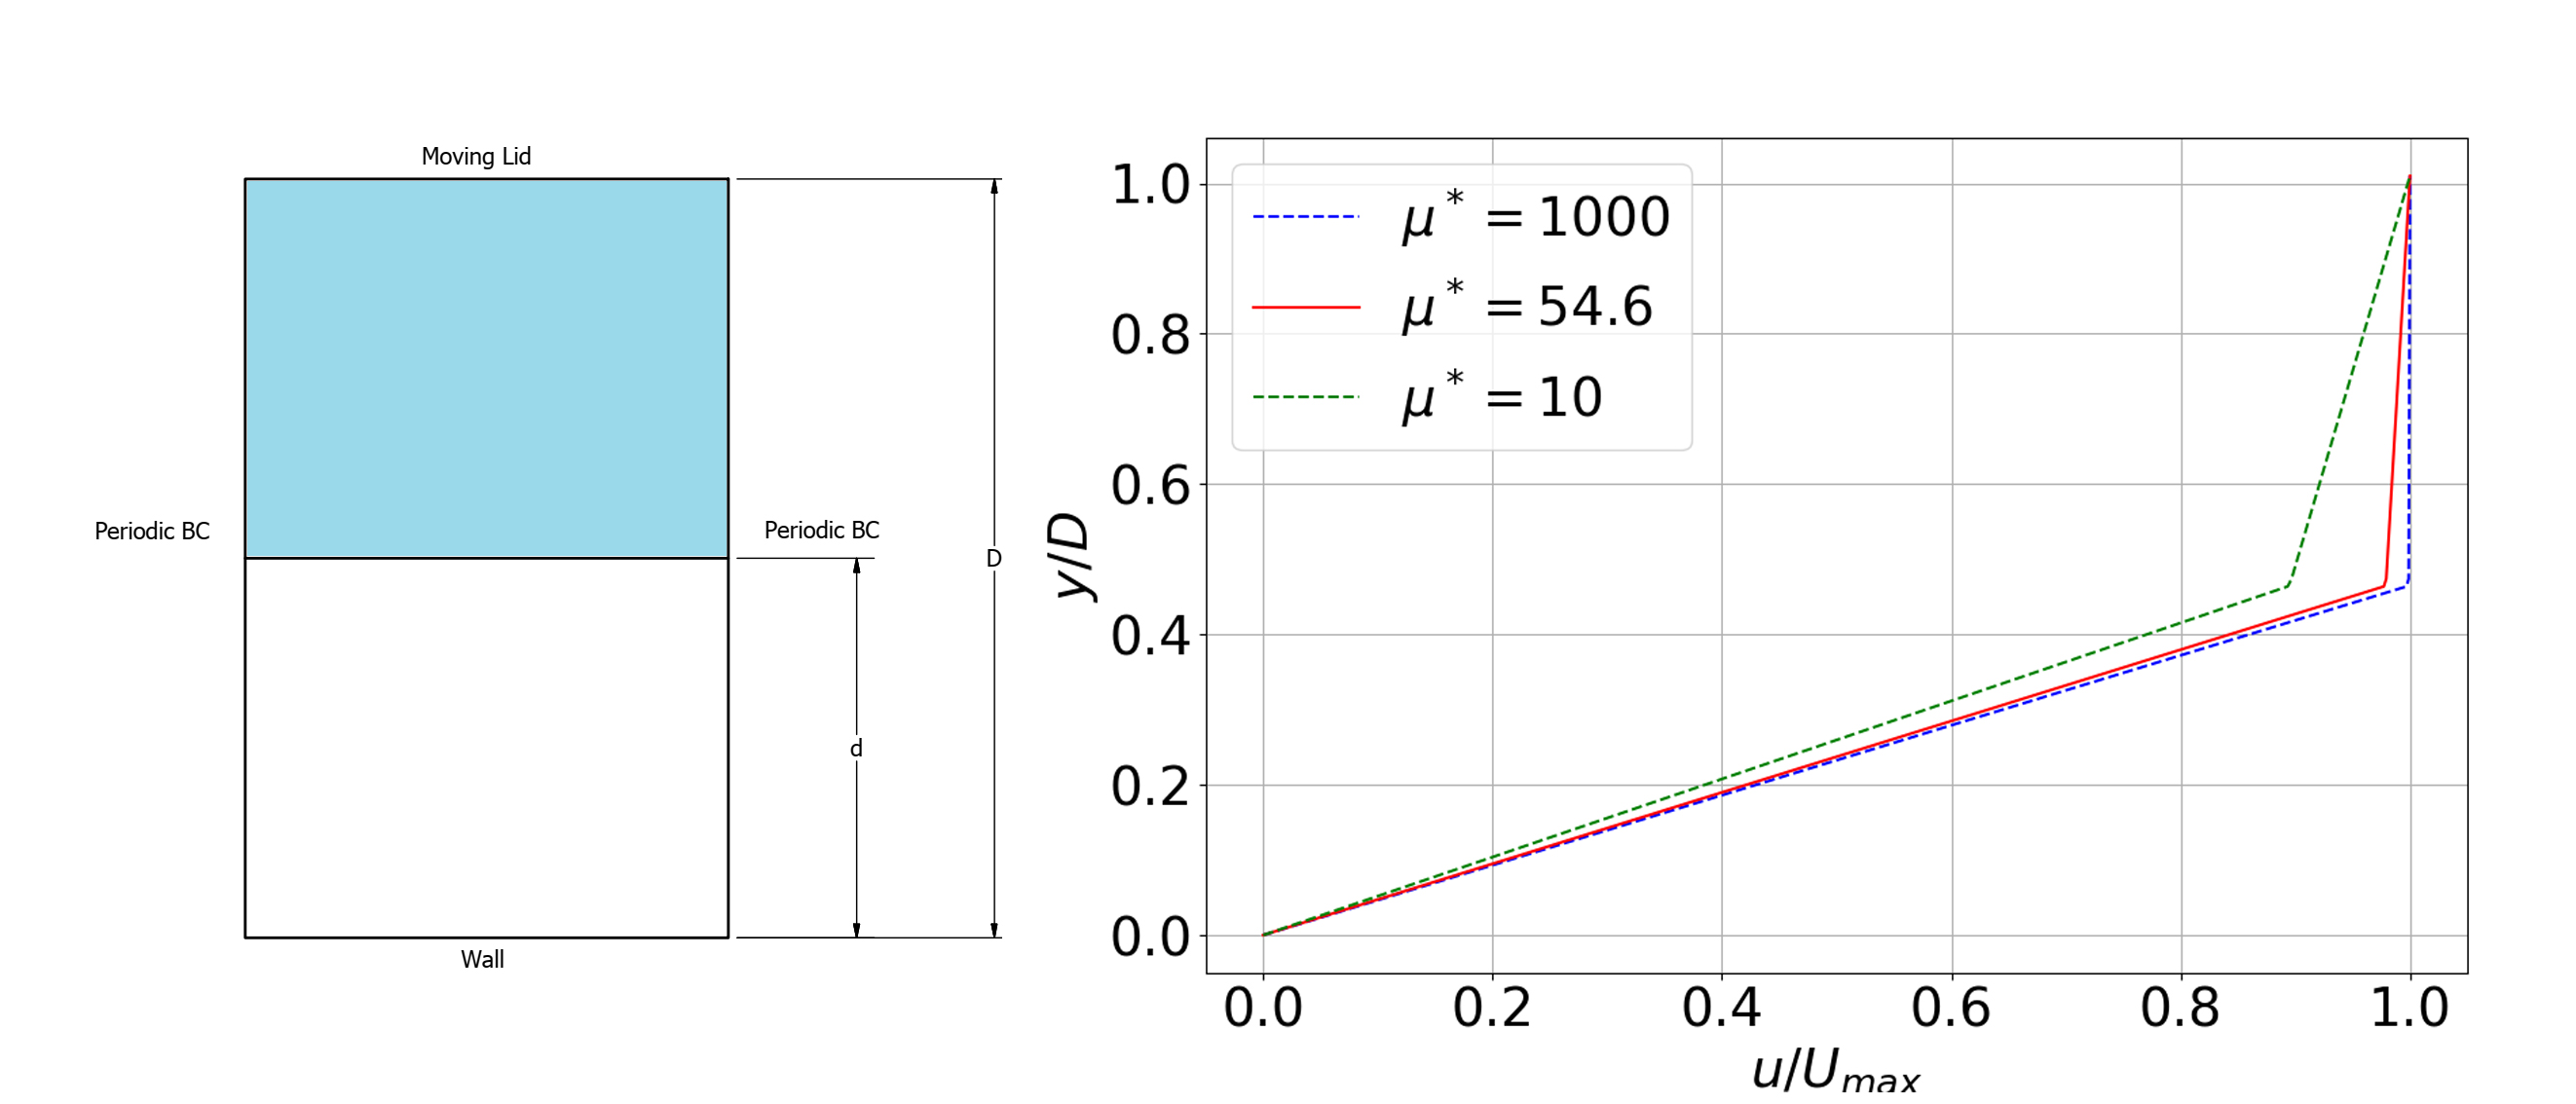
\includegraphics[width= 1 \textwidth]{Images/Couette_z_u_profile.jpg} 
   \caption{Two phase Coutte flow: \newline
   influence of $ \mu^*$ on velocity slip between phases}
   \label{fig:Couette_z_u_profile}
\end{figure}
\columnbreak 
In \cref{fig:Couette_z_u_profile} we can observe that for $\mu^*=1000$  the velocity profile resembles a perfect slip condition. %, which is consistent with \cite{Cheng2009}.
In the case of a water-air interface, $\mu^*_{water-air}=54.6$, thus the common simplification of the interface by a slip BC seems to be justified with $ \sim 2\%$ error.
%A similar conclusion can be drawn from Choi et al. \cite{Choi2003} who showed experimentally that the apparent slip length increases approximately linearly with shear rate.
\end{multicols}

\begin{multicols}{2}

\begin{figure}[H]
   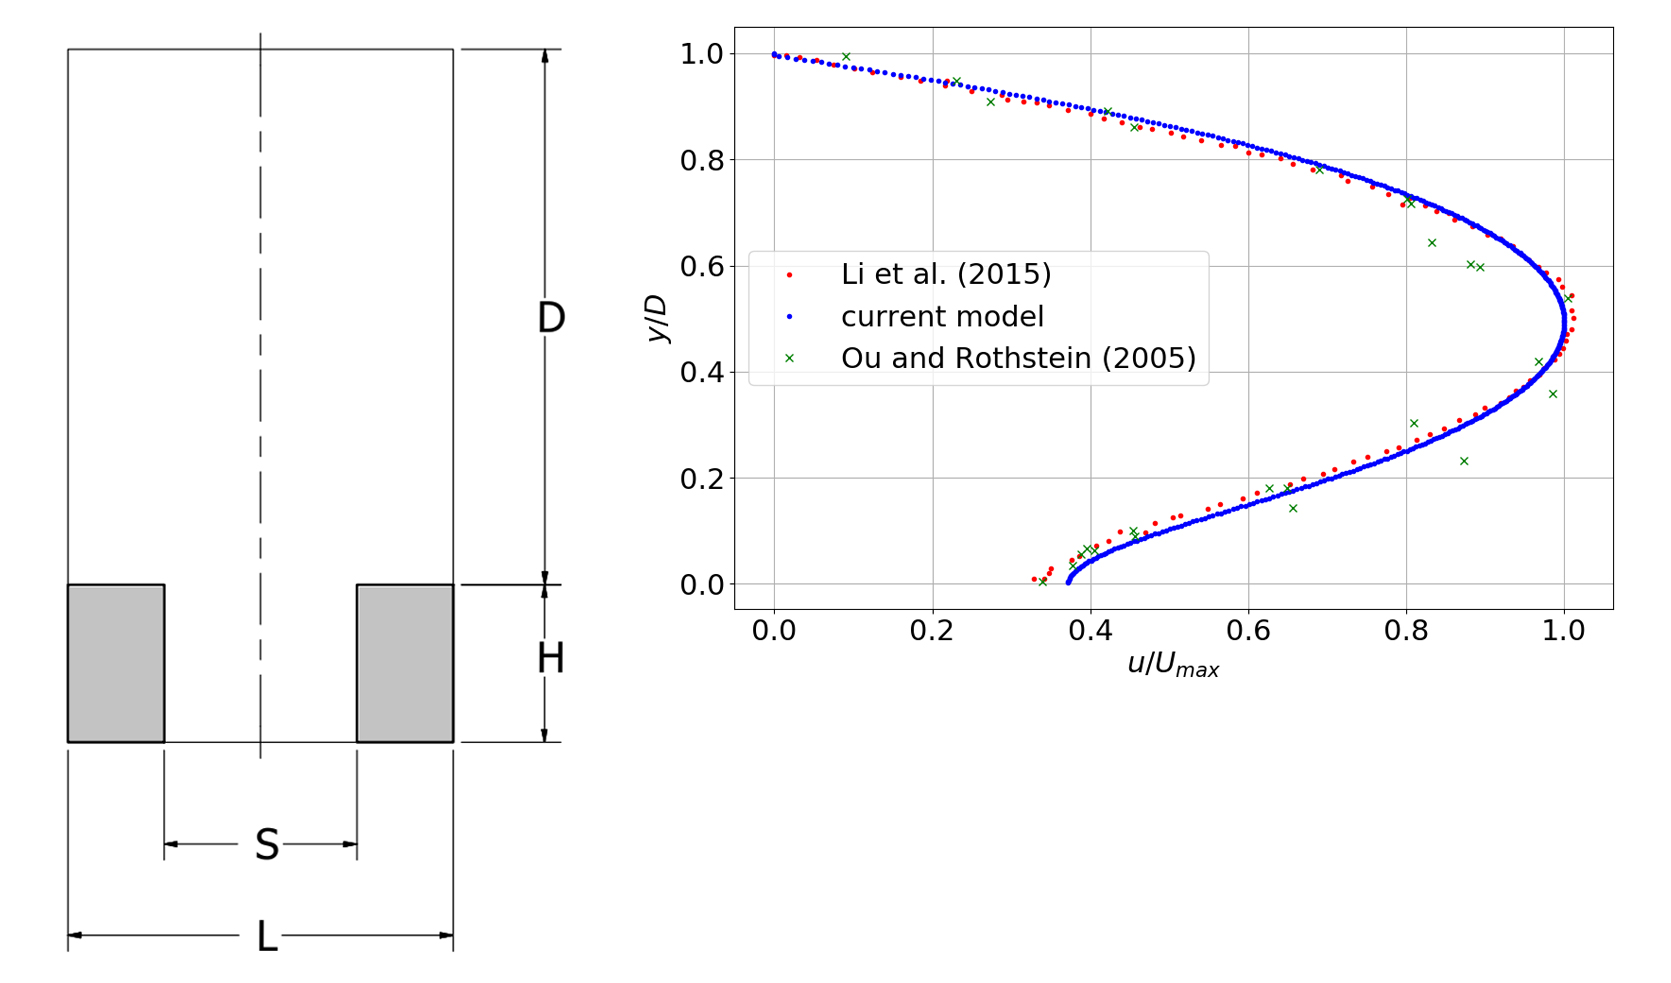
\includegraphics[width= 1 \textwidth]{Images/kanal_z_u_profile.jpg} 
   \caption{Dimensionless velocity profile at the center of the air pocket $\rho^∗ = \mu^∗ = 54:6$ }
   \label{fig:kanal_z_u_profile}
\end{figure}
\columnbreak 
A typical geometry of a simple, periodic super hydrophobic surface is shown in \cref{fig:kanal_z_u_profile}. 
Gentle filling of the geometry with water keeps the air bubble entrapped between solid posts (grey). 
Finally, the flow can be driven by gravity or a pressure difference.
Having compared the velocity profiles above the entrapped air, we conclude that our results are in agreement with the ones obtained by other researchers.
\end{multicols}
\end{block}
\end{column}


\begin{column}{.46\textwidth}
\begin{block}{Summary}
In this work, a phase-field LBM was proposed with an implementation of the collision routine in the central moment space, 
which improves the model performance in terms of both Galilean invariance and discretization errors. 
Presented model has been successfully validated against both analytical and experimental benchmarks.
Additionally, the LBM is relatively easy in implementation and able to handle complex geometries such as porous media or rough surface. Computations are performed locally, thus the algorithm can be parallelized in a straightforward manner.  

\begin{center}
\textbf{Treatment of an air-water interface}
\end{center}

\begin{multicols}{2}
\textbf{Common simplifications}
 \begin{list}{•}{}
\item rigid surface
\item perfect slip 
\item seek of an ideal SHS may leads to a trivial solution - two phase Coutte flow 
 \end{list}  
\columnbreak 
\textbf{What we achieved}
 \begin{list}{•}{}
  \item simulations of a deformable air-water interface at micro scale
  \item applicable to fluids having high density ratio
  \item able to capture complex geometry
 \end{list}  
\end{multicols}

%\begin{table}[H]
%\begin{tabular}{ll}
%\hline
%\multicolumn{2}{c}{\textbf{Treatment of air-water interface}} \\
%\multicolumn{1}{c}{\textbf{Common simplifications}} & \multicolumn{1}{c}{\textbf{What we achieved}} \\ \hline
%rigid surface   & simulations of a deformable air-water interface at micro scale    \\
%perfect slip  & applicable to fluids having high density or viscosity ratio    \\
%seek of an ideal SHS may leads to a trivial solution - two phase Coutte flow & able to capture complex geometry \\ \hline
%\end{tabular}
%%\hspace{0.25\textwidth}
%\end{table}

\end{block}

\end{column}
\end{columns}

%\begin{block}{References}
%\bibliographystyle{sbc}
%\bibliography{library.bib}
%\end{block}

\end{frame}
\end{document}

%%%%%%%%%%%%%%%%%%%%%%%% TEMPLATE %%%%%%%%%%%%%%%%%%%%%%%%

%\begin{columns}[T]
%\begin{column}{.46\textwidth}

%\begin{block}{Algorithm fluid}
%\lipsum[1]
%\end{block}
%\end{column}
%
%
%\begin{column}{.46\textwidth}
%\begin{block}{Algorithm fluid}
%\lipsum[2]
%\end{block}
%\end{column}
%\end{columns}
%%%%%%%%%%%%%%%%%%%%%%%% END OF TEMPLATE  %%%%%%%%%%%%%%%%%%%%%%%%

%%%%%%%%%%%%%%%%%%%%%%%% TEMPLATE %%%%%%%%%%%%%%%%%%%%%%%%
%\begin{block}{Sample...}
%\lipsum[1]
%\end{block}
%\begin{multicols}{2}
%\lipsum[2]
%\columnbreak 
%\lipsum[3]
%\end{multicols}
%%%%%%%%%%%%%%%%%%%%%%%% END OF TEMPLATE  %%%%%%%%%%%%%%%%%%%%%%%%
